\documentclass[10pt, aspectratio = 169]{beamer}
% Use package form https://github.com/tgodfrey0/soton-beamer/tree/main
% Theme choice
\usetheme{Soton}
\usecolortheme{default}

% Title page information
\title{Machine Learning with graphs - Project Defense}
\subtitle{Delaunay Graph: Addressing Over-Squashing and Over-Smoothing Using
Delaunay Triangulation\\
by Attali H., Duscaldi D. and Pernelle N. \texorpdfstring{\cite{attali2024delaunay}}}

\author{Edwin Roussin and Tristan Waddington}
\supervisor{Supervised by Jhony H. Giraldo}
\institute{IP-Paris, CEMST}
\date{26/03/2025}

\setTitleLogoRight{figures/CEMS Terre_nouveau logo792x445px.png}
% \setTitleLogoCentre{robot.pdf}
\setTitleLogoLeft{figures/ipparis.png}
\setLogo{figures/ipparis.png}
% \setColourScheme{50}{85}{234}
% \setProgressBarOff
% \setFrameNumbersOff

\begin{document}

% Title slide
\begin{frame}
    \titlepage
\end{frame}

% Introduction
\begin{frame}
    \frametitle{Introduction}
    \begin{block}{Delauney triangulation}
    Reconstruct a graph completely from features using the Delaunay triangulation.

    $\Rightarrow$ Avoid over-smoothing and over-squashing.
    \end{block}
    
    \begin{figure}
        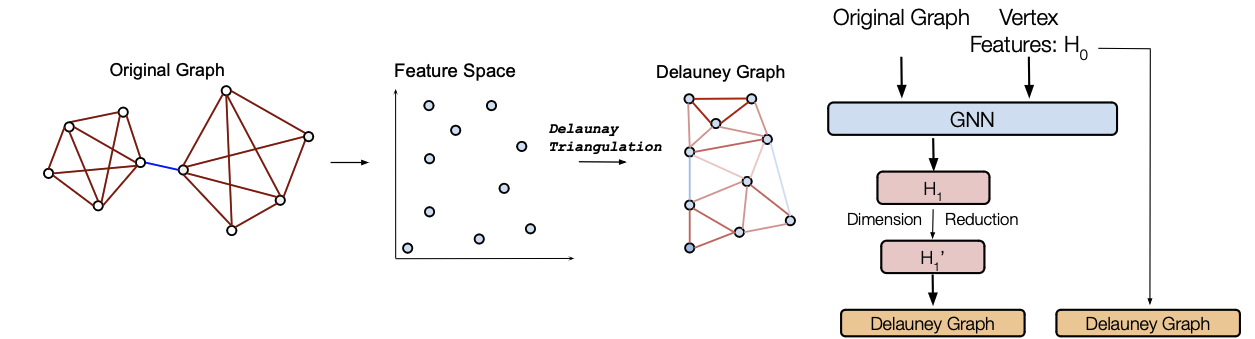
\includegraphics[width=0.6\textwidth]{figures/Delaunay-Rewiring.png}
        \caption{Illustration of the Delaunay [Attali al., 2024] \cite{attali2024delaunay}}
    \end{figure}
\end{frame}


% Automatic Outline slide
\begin{frame}
    \frametitle{Outline}
    \tableofcontents
\end{frame}

% =====================================
% Issues with graph rewiring
% =====================================
\section{Issues with graph rewiring}

\subsection{Over-Squashing}
\begin{frame}
    \frametitle{Over-Squashing}
    
    \begin{columns}
        \begin{column}{0.4\textwidth}
            \begin{figure}
                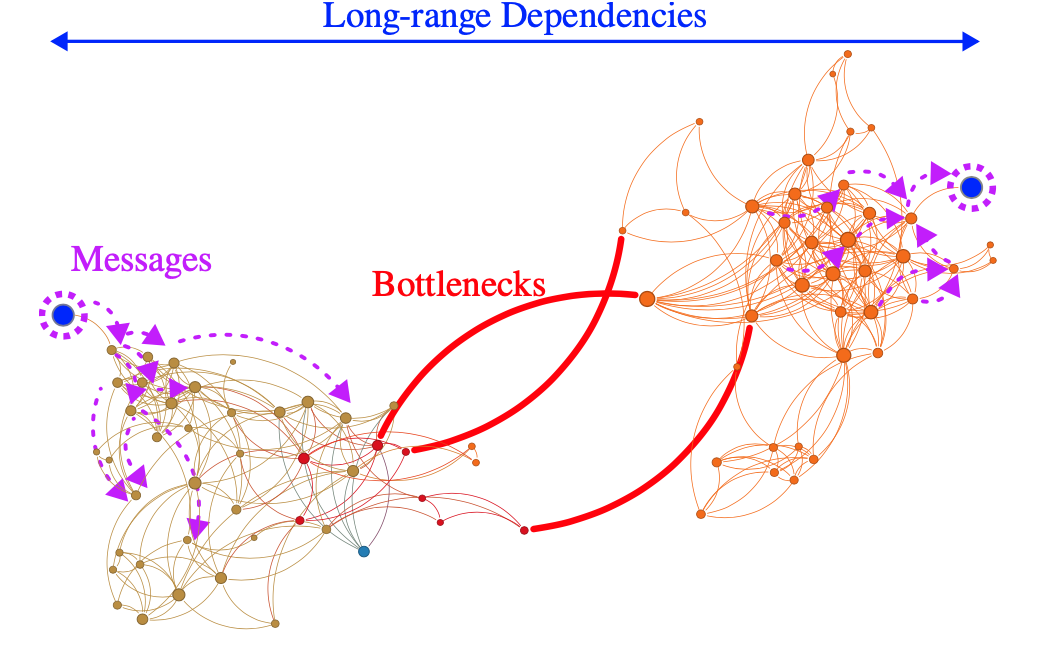
\includegraphics[width=0.99\textwidth]{figures/over_squashing_Girarldo.png}
                \caption{Illustration of Bottlenecks [Giraldo, Lecture GNNs, 2025]}
            \end{figure}

        \end{column}    

        
        \begin{column}{0.4\textwidth}

        \end{column}
    \end{columns}

  

\end{frame}

\subsection{Over-Smoothing}
\begin{frame}
    \frametitle{Over-Smoothing}
    \textbf{Avoid over-smoothing in preventing the embedding to become the same:}:
    \begin{itemize}
        \item \textbf{Normalization} with PairNorm [Zaho, 2020]\cite{zhao2020pairnorm}.
        \item \textbf{Rewiring} Drop edges, at random [Rong, 2019]\cite{rong2019dropedge} 
              or in finding the potential good ones [Giraldo, 2023]\cite{Giraldo_2023}
    \end{itemize}

    \begin{alertblock}{Over-smoothing and over-squashing are intrinsically related}
        Inevitable trade-off between these two issues, as they cannot be alleviated simultaneously.
    \end{alertblock}

\end{frame}

% =====================================
% Key technical novelty of the paper
% =====================================
\section{Key technical novelty of the paper}

\subsection{Theoretical Analysis}



\begin{frame}
    \frametitle{Theoretical analysis}
    \begin{columns}
        \begin{column}{0.4\textwidth}
        \begin{block}{Delaunay rewiring}
            \begin{itemize}
                \item Is an extreme 2 steps rewiring method.
                \item Where all edges are rebuilt during training from a umap embedding to triangles.
                \item Then mixed with the original edges of the graph.
            \end{itemize}
        \end{block}
        \end{column}
        \begin{column}{0.4\textwidth}
            \begin{figure}
                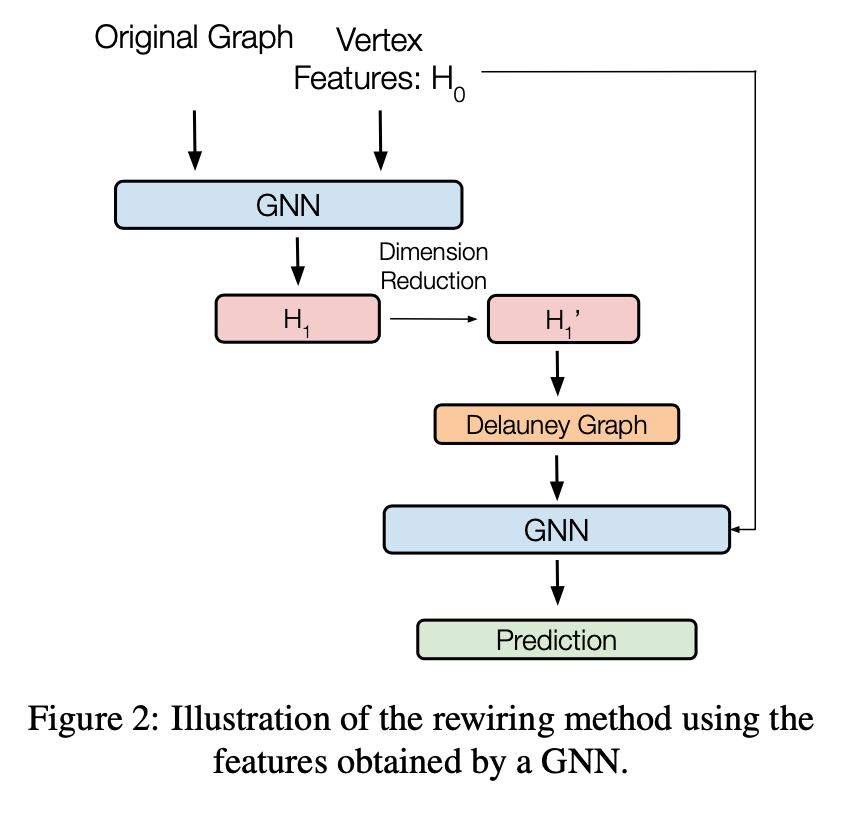
\includegraphics[width=0.99\textwidth]{figures/Rewiring_method.png}
                %\caption{Illustration of the Delaunay [Attali al., 2024] \cite{attali2024delaunay}}
            \end{figure}
            
        \end{column}
    \end{columns}

\end{frame}

\begin{frame}
    \frametitle{Theoretical analysis}
    \begin{figure}
        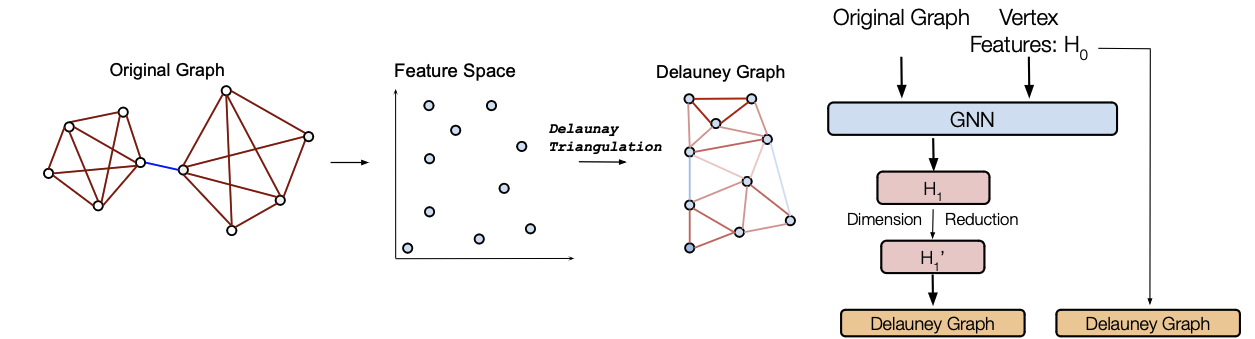
\includegraphics[width=0.6\textwidth]{figures/Delaunay-Rewiring.png}
        \caption{Illustration of the Delaunay [Attali al., 2024] \cite{attali2024delaunay}}
    \end{figure}

\end{frame}


% =====================================
% Experiments
% =====================================
\section{Experimental Evaluation}
\subsection{Methodology}
\begin{frame}
    \frametitle{Methodology}
    Aim  to reproduce as closely as possible the experiments of the authors. 
    \begin{itemize}
        \item Get same datasets, and preprocess them.
        \item Train the models with the same hyperparameters.
        \item Finally, we evaluate the models with the same metrics.
    \end{itemize}

        
\end{frame}

\subsection{Results}
\begin{frame}
    \frametitle{Results}
    \begin{exampleblock}{Text Dataset preparation}
        \begin{itemize}
            \item Text8 (English Wikipedia) processed.
            \item OpenWebText (GPT2 training material) processed in 18 hours.
            \item train/validation/test split according to experimental methodology.
        \end{itemize}
    \end{exampleblock}

    \begin{alertblock}{We were unable to run the models}
        \begin{itemize}
            \item Training impossible on our machines (size of model).
            \item Does not work on Colab (tensorflow numpy2 incompatibilities).
            \item No trained model shared by the authors.
        \end{itemize}
    \end{alertblock}
    
\end{frame}

\subsection{Discussion}
\begin{frame}
    \frametitle{Discussion}
    \textbf{We faced huge challenges}
    \begin{itemize}
        \item Graphs
    \end{itemize} 
    
    \textbf{Future paper that will be explored in the report:}
    \begin{itemize}
        \item \textit{Cayley Graph Propagation} by JJ Wilson, Maya 
        Bechler-Speicher, Petar Veličković \cite{wilson2024cayleygraphpropagation}
    \end{itemize}
\end{frame}

% =====================================
% Conclusion
% =====================================
\section{Conclusion}
\begin{frame}
    \frametitle{Conclusion}
    \begin{itemize}
        \item Cannot confirm the results o
        \item Not able to reproduce.
        \item Hard time digging in code and documentation.
    \end{itemize}

    \begin{block}{Do you have any question?}
        
    \end{block}
\end{frame}

% Automatic bibliography
\begin{frame}
    \frametitle{References}
    \scriptsize
    \bibliography{references}
    \bibliographystyle{plain}

\end{frame}

% =====================================
% Additional slides
% =====================================

\end{document}